
\noindent\begin{minipage}{\textwidth}
    \begin{table}[H]
        \centering
        \caption{Hiperparâmetros e Resultados do Melhor Modelo - vgg\_v11\_AM\_opt\_aug}
        \vspace{0.2cm}
        \resizebox{\textwidth}{!}{%
            \begin{tabular}{ll | lrrr}
                \hline
                \multicolumn{2}{c|}{\textbf{Hiperparâmetros}} & \multicolumn{4}{c}{\textbf{Métricas por Classe}} \\ \hline
                \textbf{Parâmetro} & \textbf{Valor} & \textbf{Classe} & \textbf{Precisão} & \textbf{Recall} & \textbf{F1-Score} \\ \hline
    Agendador (Patience) & 7 & 31.2 & 0.1645 & 0.4513 & 0.2411 \\ 
Agendador de LR & ReduceLROnPlateau & 31.3 & 0.1376 & 0.0743 & 0.0965 \\ 
Architecture & vgg19\_bn & 31.4 & 0.0816 & 0.0190 & 0.0309 \\ 
Augmentation (Método) & None & 32.3 & 0.1713 & 0.3163 & 0.2222 \\ 
Batch Size & 32 & 32.4 & 0.0000 & 0.0000 & 0.0000 \\ 
Decaimento de Peso (WD) & 0.0032 & 33.3 & 0.1532 & 0.0881 & 0.1118 \\ 
Dropout & 0.4754 & 41.4 & 0.0000 & 0.0000 & 0.0000 \\ 
Função de Perda & CrossEntropyLoss & 41.5 & 0.0000 & 0.0000 & 0.0000 \\ 
Hidden Units & 512 & 42.4 & 0.0909 & 0.0147 & 0.0253 \\ 
Label Smoothing & 0.0000 & 44.4 & 0.0000 & 0.0000 & 0.0000 \\ 
\cline{3-6} 
Otimizador & SGD & \textbf{Média (Macro)} & 0.2864 & 0.3238 & 0.2637 \\ 
Taxa de Aprendizado (LR) & 2.09e-04 & \textbf{MCC} & \multicolumn{3}{c}{0.2267} \\ 
Unfreeze Layers & 6 &  & & &  \\ 
            \hline
            \end{tabular}%
        }
    \end{table}

    \begin{figure}[H]
        \centering
        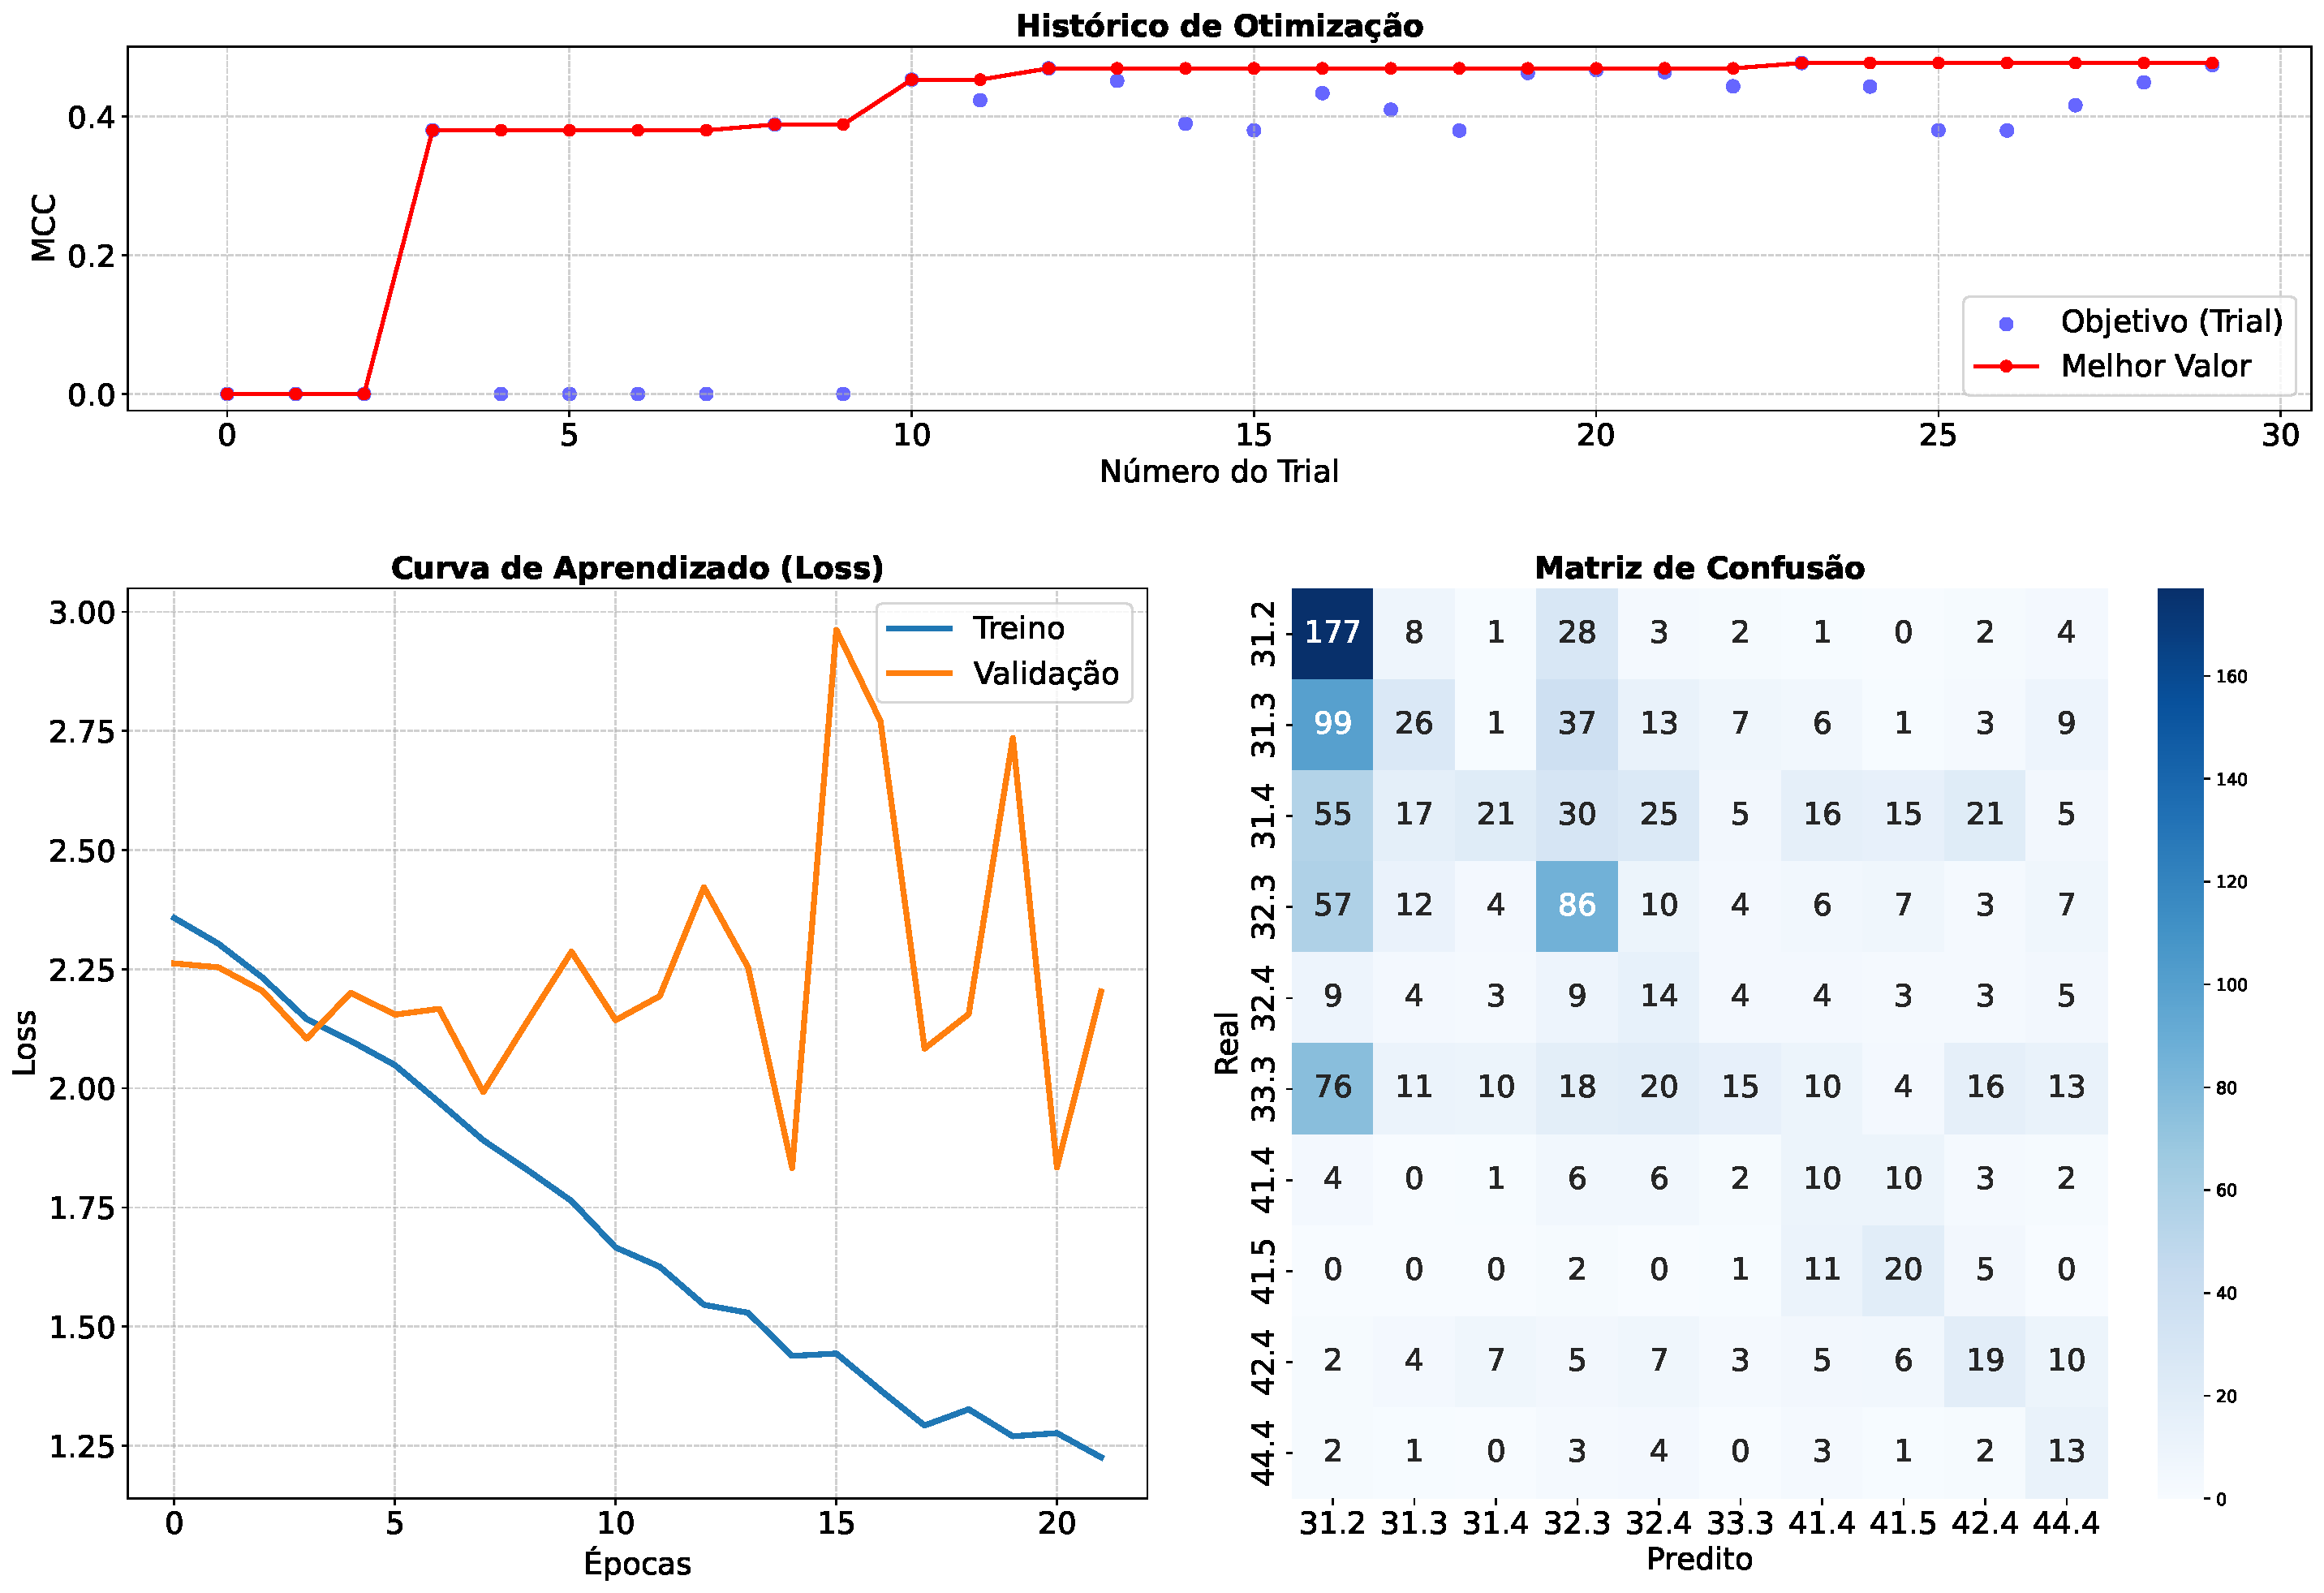
\includegraphics[width=0.85\textwidth]{tex/appendix/experiments/vgg_v11_AM_opt_aug/dashboard_consolidado.pdf}
        \caption{Histórico de Otimização, Curvas de Aprendizado e Matriz de Confusão - vgg\_v11\_AM\_opt\_aug}
    \end{figure}
\end{minipage}
\clearpage
